\section{Theoretical and Simulation Analysis}
\label{sec:analysis}

In order to compare \textit{side by side}, we'll discuss the theoretical and simulation analysis at the same time.

However, one has to present the circuits implemented on the AC DC converter in order to fully understand the simulation. The constants values used during the theorectical analysis are expressed in the table below.

\begin{table}[h]
    \centering
    \begin{tabular}{|l|c|c|}
    \hline
    {\bf Name} & {\bf Value} & {\bf Units} \\ \hline
    $V_{ON}$\footnotemark & $0.63158$ & $V$ [Volts] \\ \hline
    $I_s$ & $1\cdot10^{-14}$ & $A$ [Amperes] \\ \hline
    $R_{env}$ & $140$ & $k\Omega$ [kOhms] \\ \hline
    $R_{vreg}$ & $120$ & $k\Omega$ [kOhms] \\ \hline
    $C$ & $600$ & $\mu F$ [$\mu$Farad] \\ \hline
    $V_{in}$ & $201.135$ & $V$ [Volts] \\ \hline
    $N_i$ & $1.14351$ & Transformer Ratio \\ \hline
    $V_T$ & $25.88794\cdot10^{-3}$ & V [Volts]\\ \hline
    $\eta$ & $1$ & Constant \\ \hline
    \end{tabular}
    \caption{Constants Values}
    \label{tab:constants}
\end{table}
\footnotetext{$V_{ON}$ value is computed using \textit{Ngspice} results for $V_{out}$. By definition, $V_{ON}=\frac{V_{out}}{N_{diodes}}$}

\subsection{Envelope Detector Circuit}
\label{subsec:stat}

Firstly, we must discuss the first half of the circuit that was used. A Full Wave Bridge Rectifier along side a Resistor and a Capacitor in paralell were used to envelope the $V_{in}$ sinusoidal wave. An important characteristic we should bear in mind is that, because it is best wanted to have the minimum ripple possible, the time constant $\tau$ of the capacitor discharge should be as high as possible, so that $V_o$ stays as constant as possible during this time. To achieve this, because $\tau=RC$, a simple solution is to increase the resistor impedance ($R$) and the capacitor capacity ($C$). Of course, a more intelligent solution is to use a full-wave bridge rectifier insted of a half-wave, so that the time of discharge of the capacitor is decreased to half (the frequency of the wave is doubled). It should be noted that $V_{in}$ is the transformed voltage from the plug: $\frac{230}{N_i}$. 

A scheme of this circuit is presented below.

\begin{figure}[h]
    \centering
    \includegraphics[scale=0.4]{Envelope.pdf}
    \caption{Envelope Detector Circuit}
    \label{fig:envelope_detector}
\end{figure}

\clearpage

\subsection{Voltage Regulator Circuit}

The second half of the AC/DC converter is composed by a Voltage Limiter in series with a resistor, both in parallel to the Envelope Detector. The input voltage of this circuit is $V_o$ of the Envelope Detector. The purpose of this circuit is, besides limiting the voltage, atenuating the rough ripple of $V_o$, see equation (4). This circuit is analysed in the following way: first, one should separate in DC and AC components. The DC simulation using the diode model described yields that the condition $V_o=N\cdot V_{ON}$ which ensures forward bias at all the diodes, and so, each one can be substituted by an equivalent voltage source $V_{ON}$. Of course, if $V_o<N\cdot V_{ON}$, the output voltage $V_{out}$ is $V_o$, since the diodes are off, which means the circuit can be considered to be open. The AC incremental analysis is explained in further detail in the next section.

\begin{figure}[h]
    \centering
    \includegraphics[scale=0.5]{Regulator.pdf}
    \caption{Voltage Regulator Circuit}
    \label{fig:Regulator}
\end{figure}

In conclusion, when we merge these two circuits, we end up with our AC/DC converter in Figure \ref{fig:circuitol3}.

\clearpage

\subsection{Theoretical Analysis}
\label{subsec:Req}

For the Theoretical approach, we used the Ideal Model + Voltage Source, $V_{ON}$. This choice was made because it gives a pretty good approximation of the Diode Equation, and the latter is more time-consuming due to the need of solving numerically non-linear equations.

By applying KVL to the Envelope Detector, either in its positive cycle (when $D_1$ and $D_3$ are ON) or its negative cycle (when $D_2$ and $D_4$ are ON), we end up with, 

\begin{equation}
    V_o=-2V_{ON}+V_{in}
\end{equation}

The diodes, however turn off when the current on the resistor, $i_R$, equals the current on the capacitor, $i_C$, which leads to,

\begin{equation}
    \frac{Acos(\omega t|_{OFF})-2V_{ON}}{R_{eq}}=A\omega sin(\omega t|_{OFF})
\end{equation}
where $R_{eq}=R_{env}||R_{vreg}$

Solving this equation yields $t_{OFF}$, which allows us to know when the diodes turn off and an exponential decay, due to the the capacitor discharge, occurs. 

\begin{equation}
    V_o=V_o|_{t_{OFF}}e^{-\frac{t-t_{OFF}}{R_{eq}C}}
\end{equation}

The Diodes turn on again when $V_{in}=V_o+2V_{ON}$. With this non-linear equation one can estimate $t_{ON}$. By knowing that this behaviour repeats in each half wave period, we have all the needed information to theoricaly preview the behaviour of this circuit.

For the Voltage Regulator, we perform a DC + AC analysis, the latter using incremental analysis. If we separate both components, we have $V_o=V_O+v_o$

Concerning DC analysis, if $V_O>N \cdot V_{ON}$, then $V_O=N \cdot V_{ON}$, where $N\equiv$ the number of diodes.

Concerning the incremental analysis, 

\begin{equation}
    v_{out}=\frac{N\cdot r_d}{N\cdot r_d + R_{vreg}}v_o
\end{equation}
where $r_d\equiv$ diode resistance using incremental analysis.

\begin{equation}
    r_d=\frac{\eta V_T}{I_s e^{\frac{V_D}{\eta V_T}}}
\end{equation}

where $V_T=\frac{kT}{q}$, $k\equiv$ \textit{Boltzmann} constant, $T\equiv$ temperature (in K) and $q\equiv$ electron charge.

By making $r_d$ smaller, it is expected that the $v_{out}$ ripple should go down. A simple solution to decrease this resistance is simply to add layers  of parallel diodes in series, so that $I_s$ decreases if we take the relation for diodes in parallel: $I_{s_{eq}}=N \cdot I_s$. However, as we discuss in further detail in \ref{sec:merit}, it led us to a worse quality/cost ratio.

\pagebreak
\subsection{Comparison}
\label{subsec:comparison}

We are now ready to make a comparison of the two approaches.

Let us start by seeing the overall panorama with the plots of $V_{in}$, $V_{o}$ and $V_{out}$ as well as the values of the deviation and ripple. We will firstly present the theoretical plots of these values, as well as a table with some important results.

\begin{figure}[h]
    \centering
  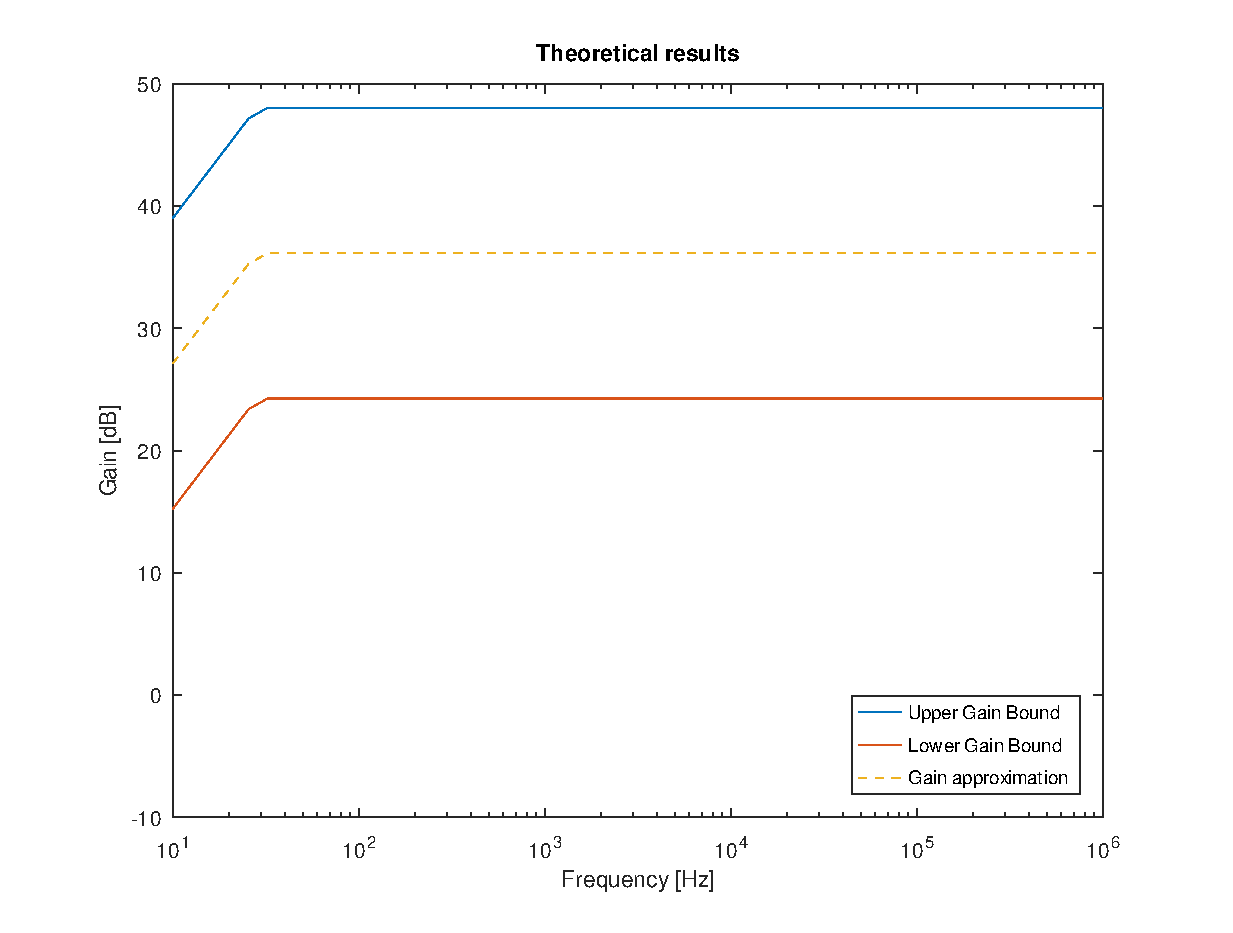
\includegraphics[scale=0.6]{theo_results.eps}
 \caption{Theoretical Results}
\end{figure}

\begin{table}[h]
    \centering
    \begin{tabular}{|l|c|}
    \hline
    {\bf Name} & {\bf Value [V]} \\ \hline
    \input{theo_table_del.tex}
    \end{tabular}
    \caption{Theoretical Values}
    \label{tab:theo_ripple_deviation}
\end{table}
\pagebreak
\begin{figure}[h]
    \centering
  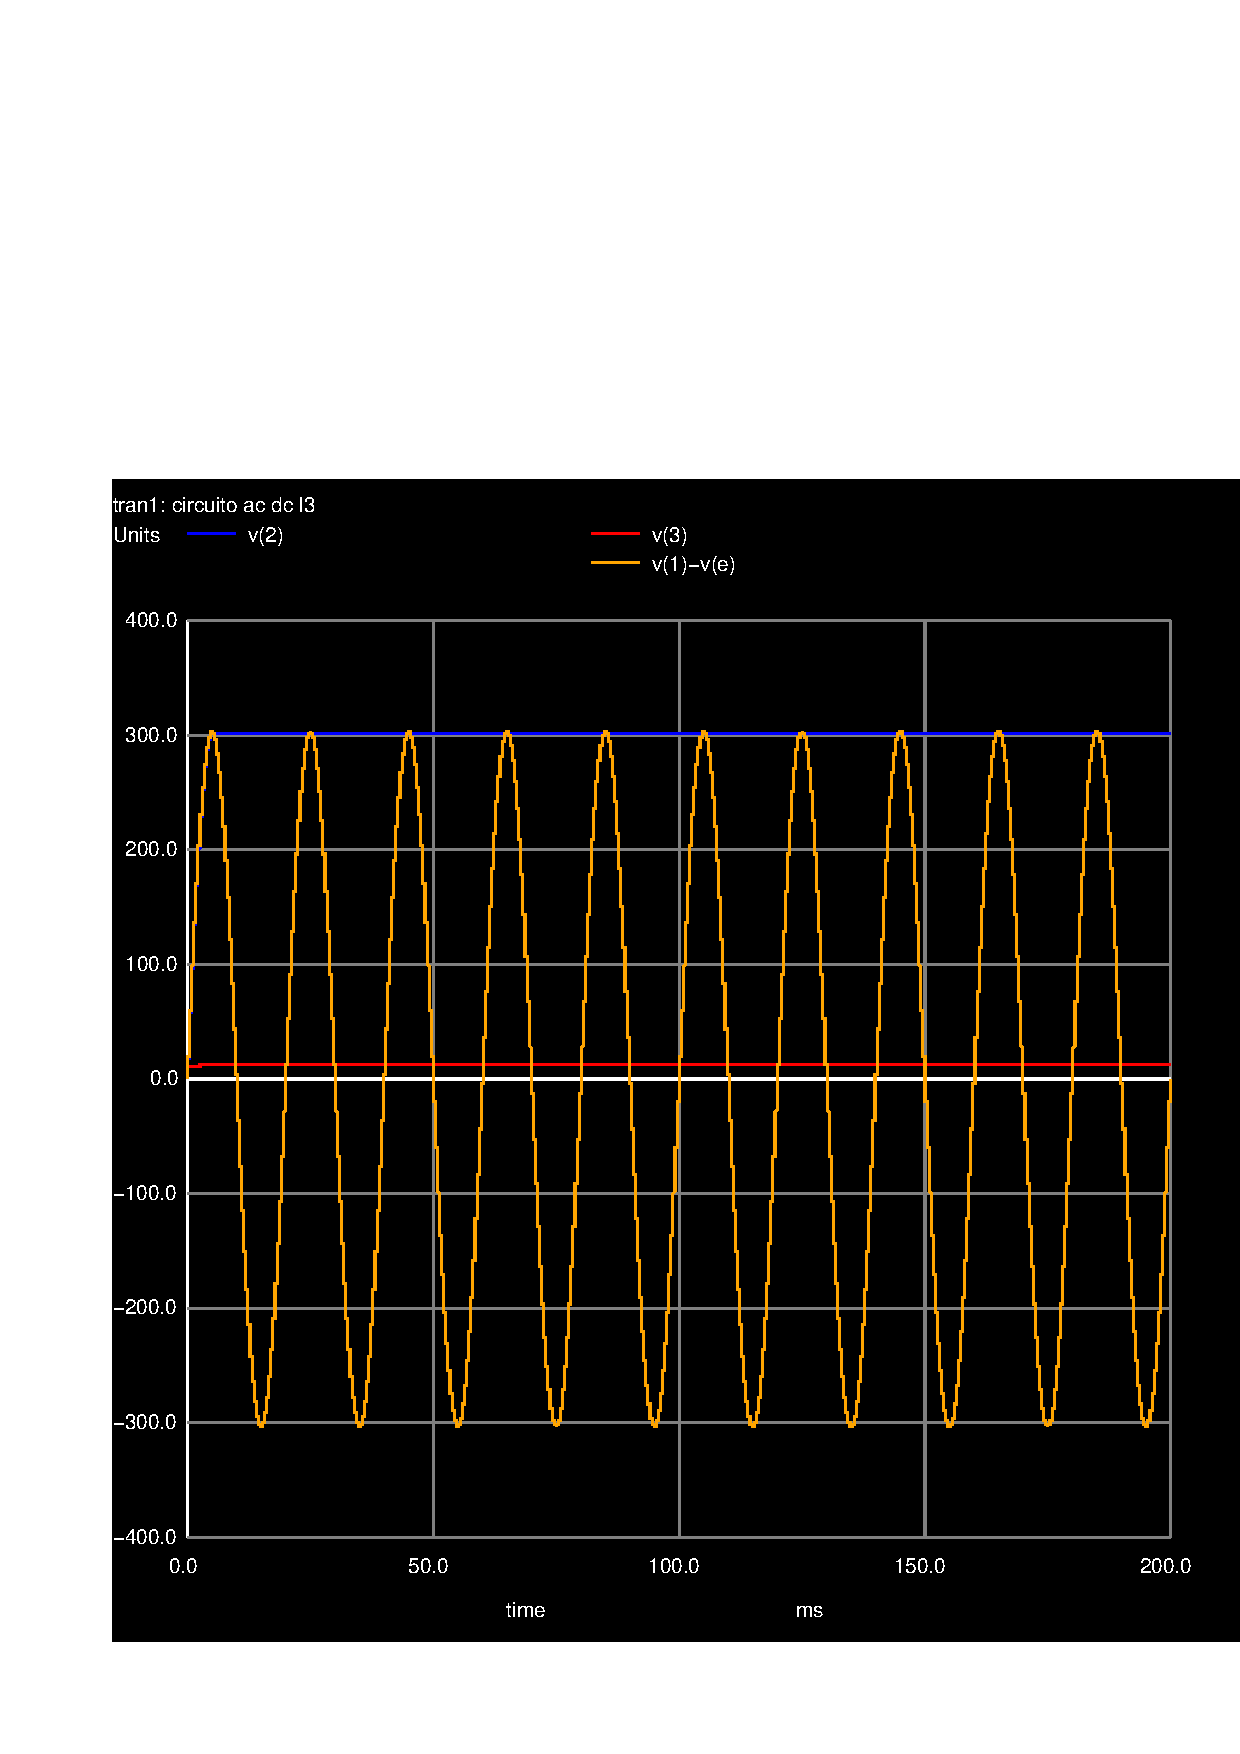
\includegraphics[scale=0.5]{exp_results.pdf}
  \caption{Simulation Results}
\end{figure}


\begin{table}[h]
    \centering
    \begin{tabular}{|l|c|}
    \hline
    {\bf Name} & {\bf Value [V]} \\ \hline
    \input{ripple_desvio_tab.tex}
    \end{tabular}
    \caption{Simulation Values}
    \label{tab:exp_ripple_deviation}
\end{table}

Let us zoom in to analyse with further detail the ripple and the deviation. Again, we firstly present the plots obtained through the theoretical analysis, followed by the Ngspice simulation.

\pagebreak

\begin{figure}[h]
    \centering
  \includegraphics[scale=0.45]{theo_ripple.eps}
 \caption{Theoretical Ripple and Deviation Results}
\end{figure}

\begin{figure}[h]
    \centering
  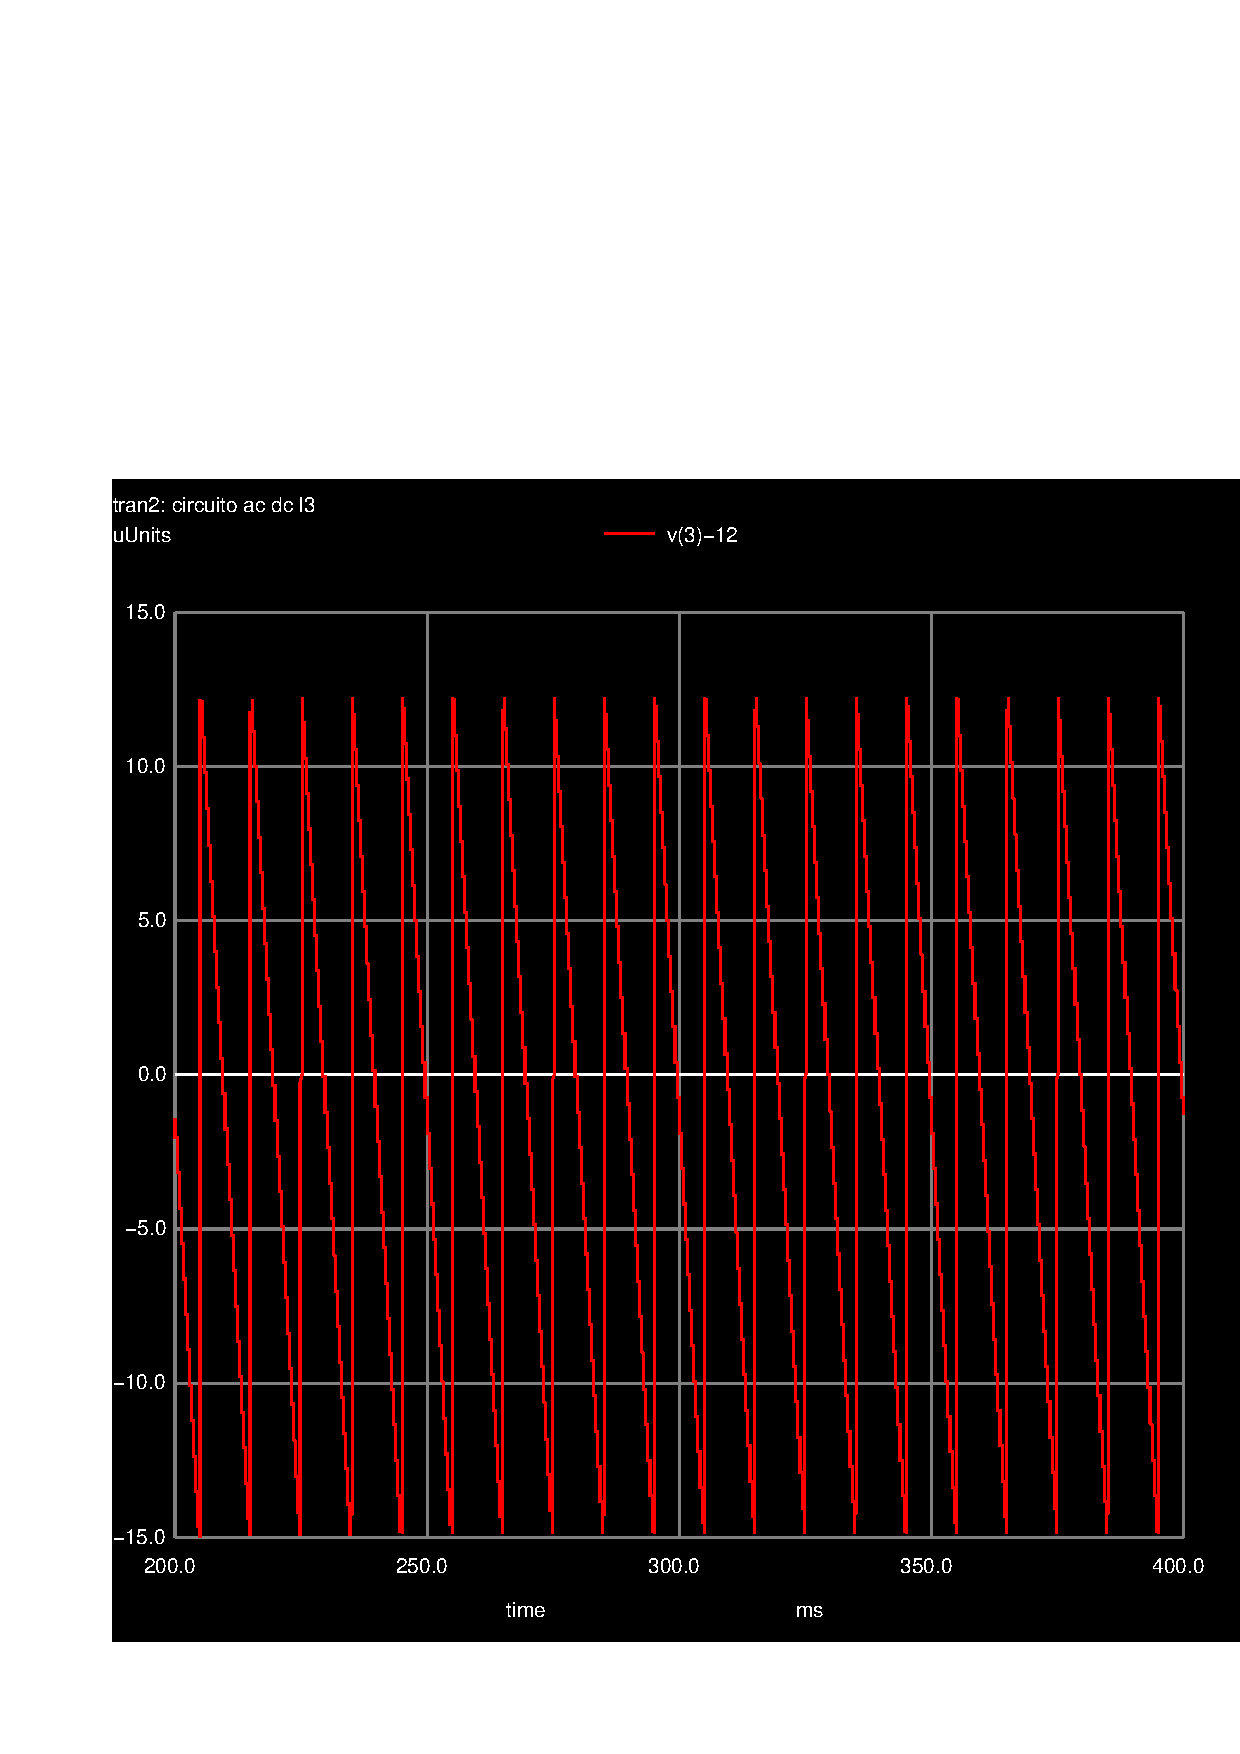
\includegraphics[scale=0.34]{exp_ripple.pdf}
  \caption{Simulation Ripple and Deviation Results}
\end{figure}

\pagebreak

The overall behaviour and shape of both plots is \textbf{similar}. As important features we can underline the fact that $V_o$ has \textbf{twice the frequency} of $V_{in}$, due to the full wave rectifier. We can also notice in both approaches an \textbf{exponential decay} due to the capacitor as seen in Section \ref{subsec:Req}.
It is important to notice that there is some kind of \textbf{distortion}, eventhough not a significant one, something expected due to the satisfying results we had.

With greater detail, we can easily realize, as seen in tables above as well as plot comparison, that the \textbf{theoretical ripple is bigger than the one presented on the simulation model}. 
However, when we experimented several circuits, sometimes we saw the opposite results. This occurance is yet just another example of the non-linearity and complexity of the model used by \textit{Ngspice}, for small differences on the circuit can alter the behaviour of diodes themselves. Eventhough this happens, both results are interesting and satisfying, for they provide a somewhat stable output.

When it comes to the deviation (offset), a value of 0V was obtained (or smaller than $1E-06$ for Ngspice represents it as 0). On the theoretical side, we had a bigger offset. This difference, again, is not surprising, because there are a lot of different parameters involved on the simulation model, and just a few on the theoretical ones. Besides, we don't know for sure the value o $V_{ON}$ used in \textit{Ngspice}, as it changes depending on the circuit. However, we approximated it to a constant by dividing the Ngspice output average by the number of diodes used, as we needed a somewhat correct value to use in the theoretical analysis.
As a remark, we can state that a deviation of 0V was a factor easier to achieve than the ripple, as we could just change $V_{in}$ (see Section \ref{sec:merit}). 

In a practical point of view, we can conclude that we had better results on \textit{Ngspice} which represents the real circuit, so its positive. This has important applications in technologies that require precision.


\clearpage

\section{Merit Results}
\label{sec:merit}

From the results obtained through the Ngspice simulation (see Section \ref{subsec:comparison}) and considering we used the data shown in Section \ref{sec:introduction}, we can compute the price and the merit using the \textit{formulae} given in the lab assignment:

\begin{table}[h]
    \centering
    \begin{tabular}{|l|c|}
    \hline
    {\bf Name} & {\bf Value} \\ \hline
    price & 2102.51\\ \hline
merit & 3.23771\\ \hline

    \end{tabular}
    \caption{Total Price and Merit}
    \label{tab:price_merit}
\end{table}

On the choice of the circuit, we started using a half wave rectifier circuit, which has a worse ratio quality/cost, which led us to choose the full wave. We also tried the option of multiple diodes in parallel, in order to reduce the resistance required.
However, we saw that it gave us a higher cost as well as higher ripple, so it was not beneficial. 

For our strategy, we opted to firstly give more attention to minimizing the ripple and the deviation, leaving the cost as a second thought. We then made small adjustments to further perfect our results, which in turn made the merit figure rise. Due to this, we saw that it was useful to increase $V_{in}$ to values close to the ones on the primary. We even realise that for some circuits, if we had a higher secondary voltage, than primary, we could have bigger merits for some circuits (\textit{e.g.} 24.5). To conclude, we began decreasing the cost until we found out the perfect compromise for us, giving the results shown in table \ref{tab:price_merit}.

